\section{Web Semántica y Ontologías}

\subsection{Open Data}

Open Data se refiere al hecho de mantener los datos publicados en internet de tal manera a cumplir con algunos requisitos para que éstos puedan ser utilizados y reutilizados en cualquier momento y desde cualquier sitio \cite{bauer2011linked}.

\subsubsection{Linked Open Data (LOD)}

Linked Open Data se enfoca en un método de publicación de datos abiertos estructurados para que puedan ser interconectados. Para lograr esto se utilizan las tecnologías como RDF, RDFa, etc. para estructurar los datos, utilizando URIs para identificar los datos individualmente. Tim Berners Lee define un modelo de 5 estrellas para clasificar e identificar el grado de publicación de datos abiertos.

\begin{table}[!htb]
\centering
\caption{Modelo de publicación de 5 estrellas}
\label{modelo-5-estrellas}
\resizebox{15cm}{!} {
\begin{tabular}{|c|l|}
\hline
\ding{72} & La información está disponible en la web (en cualquier formato) bajo una licencia abierta \\ \hline
\ding{72} \ding{72} & La información está disponible como dato estructurado (Ej. Excel en lugar de una imagen de una tabla) \\ \hline
\ding{72} \ding{72} \ding{72} & Son utilizados formatos no-propietarios (Ej. CSV en lugar de Excel) \\ \hline
\ding{72} \ding{72} \ding{72} \ding{72}  & URIs son utilizadas para que se puedan individualizar los datos \\ \hline
\ding{72} \ding{72} \ding{72} \ding{72} \ding{72}  & Los datos son enlazados con otros datos para proveer un contexto \\ \hline
\end{tabular}
}
\end{table}

\subsection{La Web Semántica}
La Web Semántica consiste en una serie de estándares y tecnologías propuestas por la W3C que promueven el uso de formatos de datos común y además de un protocolo de datos dentro de la web que nos permite compartir y reusar datos -procesables por máquinas- a través de la web. Se puede pensar la Web Semántica como una manera eficiente de representar datos en la web.

El principal problema de los datos en la web es la dificultad de su utilización a gran escala, ya que no siempre se aplican estándares de publicación de datos de manera a que facilite su procesamiento. Por otra parte, los datos enlazados a través de identificadores comunes en la web nos dan la capacidad de consultar datos de distintas fuentes y contestar preguntas complejas pero interpretar el significado de los mismos no resulta una tarea sencilla. Es por eso que las ontologías juegan un rol fundamental en la web semántica, ya que gracias a ellas podemos representar conocimiento legible y entendible por máquinas y humanos en la web.

\subsection{Ontologías}
Las ontologías son utilizadas para la representación del conocimiento, logrando así que la información esté representada de forma a que pueda ser interpretada por los computadores y humanos \cite{horrocks2011kr}. En ella se definen los conceptos de un determinado dominio, sus propiedades y relaciones entre los mismos, así también reglas para combinar términos y relaciones que permitan extender el vocabulario.
A continuación se pone a conocimiento algunas definiciones hechas acerca de las ontologías en el ámbito de sistemas de información.

\cite{gruber1993translation} definió originalmente el concepto de ontología como “Una especificación explícita de una conceptualización”. \cite{borst1997construction} definió una ontología como “Una especificación formal de una conceptualización compartida”. La definición que se eligió en este trabajo es la de \cite{studer1998knowledge}: “Una ontología se define como una especificación formal y explícita de una conceptualización compartida”.  En esta definición, conceptualización se refiere a un modelo abstracto de algún fenómeno del mundo derivado de la identificación de sus conceptos relevantes; explícita se refiere a que los tipos de conceptos y las restricciones usadas sobre ellos se definen explícitamente; formal se refiere a que la ontología debe ser “legible” por una computadora; y compartida refleja que una ontología capta un conocimiento consensual. \cite{guarino1998formal} también definió como “Un conjunto de axiomas lógicos diseñados para tener en cuenta el significado deseado de un vocabulario”.

Actualmente existen ontologías para diversos dominios de conocimiento. Algunas de las más representativas son: \textit{Simple Knowledge Organization System} (SKOS) \cite{isaac2009skos}, \textit{ Friend of a Friend} (FOAF) \cite{brickley2012foaf}, \textit{Good Relations}, \cite{hepp2008goodrelations}, MGED Ontology \cite{whetzel2006mged} y National Cancer Institute Ontology \cite{golbeck2011national}. Así también existen ontologías que no pertenecen a un dominio específico (de alto nivel) y describen conceptos generales como DOLCE \cite{Masolo02thewonderweb}.
La ontología posee varios usos en Ciencias de la Computación, como ser en el ámbito legal, médico, científico y otros, pero ganó mayor popularidad en el ámbito de la Web Semántica. A continuación veremos las ontologías en el caso de uso de la web semántica.


\subsection{Ontologías en la Web Semántica}
Uno de los principios fundamentales de las ontologías dentro de la web semántica es su reutilización y extensión, esto significa utilizar conceptos de otras ontologías, siempre y cuando sea posible, mejorando el procesamiento y la integración de datos enlazados. En lugar de duplicar esfuerzos definiendo conceptos y propiedades que ya fueron definidos en otra otología, se puede referenciar a estos elementos dentro de la nueva ontología. 

Existe una variedad de tipos de ontologías que dependen del nivel de formalidad, razonamiento y la cantidad de restricciones. En el caso más simple una ontología puede describir una jerarquía de conceptos vinculados por relaciones de subsunción y en casos más sofisticados incluir axiomas para expresar relaciones entre conceptos y restringir la interpretación pretendida.

Las ontologías para la Web Semántica son de tipo ligeras en términos de niveles de formalidad y normalmente pequeñas en tamaño haciéndolas fáciles de manejar y mantener. El poder de expresión de una ontología en la Web Semántica debe ser adecuado, el lenguaje debe ser tan expresivo como para poder describir conceptos con suficiente detalle, pero no tan expresivo como para perder la capacidad de razonamiento. Una ontología más formal o expresiva es computacionalmente más costosa, por lo que se debe encontrar un equilibrio entre los dos puntos. En la Figura \ref{img:expresividad complejidad } se puede ver el espectro de ontologías según su expresividad y complejidad computacional, en donde el lenguaje OWL y la Lógica de Descripciones se encuentran dentro de las más expresivas y costosas computacionalmente.
La capacidad de razonamiento es importante para asegurar la calidad de la ontología construida, por ejemplo, en la etapa de diseño puede ser utilizada para probar si existen conceptos contradictorios y derivar nuevas relaciones.

Las formas de representar ontologías en la Web Semántica son diversas en cuanto a lenguajes y formas de serialización, a continuación se presenta algunas de ellas.

    \begin{figure}[ht!]
    \centering
    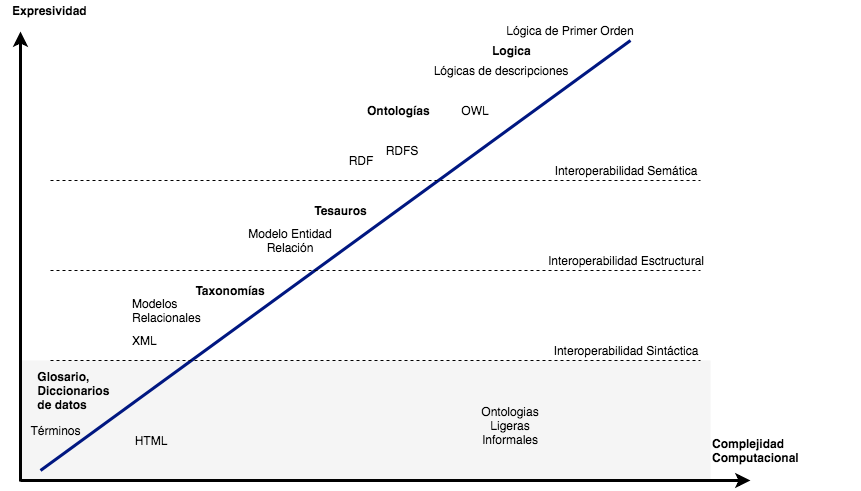
\includegraphics[width=150mm]{figuras/Diagramas-ComplejidadOntologica}
    \caption{Expresividad vs Complejidad}
    \label{img:expresividad complejidad }
    \end{figure}



\subsection{RDF y RDFS (RDF)}

Marco de Descripción de Recursos, RDF por sus siglas \textit{Resource Description Framework}  \cite{rdf}, es un framework para representar información en la Web Semántica. El lenguaje RDF forma parte de la W3C's \textit{Semantic Web Activity} y es recomendado por la W3C. El modelo de datos RDF está diseñado para que sea procesable por computadoras. 

RDF nos permite representar modelos de datos basados en grafos, los cuales son representados en triplas. Las triplas RDF contienen tres componentes:
El sujeto, que puede ser una referencia tipo URI o un Blank Node
El predicado, que es una referencia tipo URI
El objeto que puede ser una referencia tipo URI, un literal o un \textit{Blank Node}

En la Figura \ref{img:componentes rdf } se expone un grafo de ejemplo en el cual se visualizan estos tres componentes.

    \begin{figure}[ht!]
    \centering
    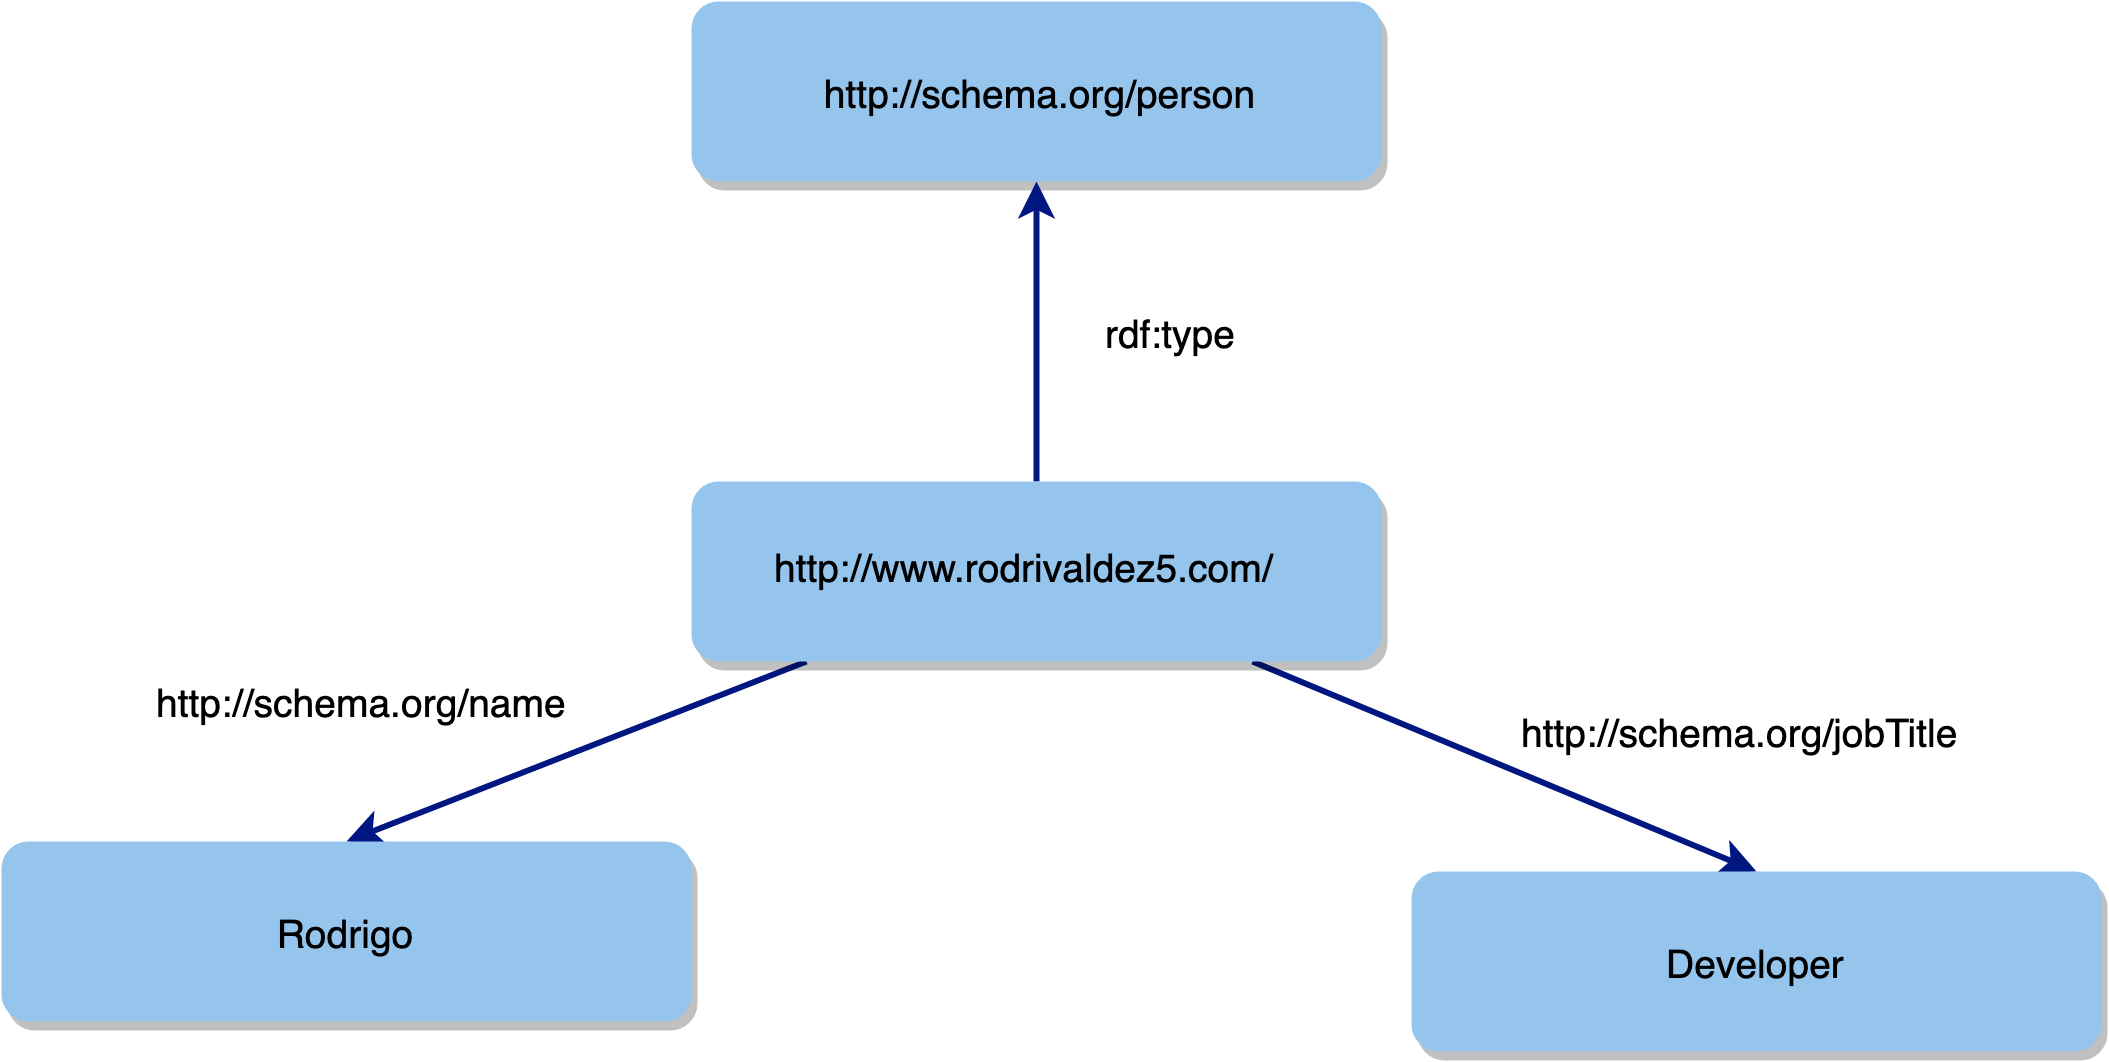
\includegraphics[width=150mm]{figuras/Diagramas-RDFGraph}
    \caption{Componentes RDF}
    \label{img:componentes rdf }
    \end{figure}
    
El sujeto es la fuente de la arista y debe ser un recurso. En RDF, un recurso puede ser cualquier cosa que sea identificable de forma única a través de un URI. Comúnmente este identificador es un URL, que es un caso especial de URI. Sin embargo, los URI son más generales que las URL. En particular, no es requerimiento que un URI se pueda utilizar para localizar un documento en Internet. El objeto de una sentencia es el objetivo de la arista. Al igual que el sujeto, puede ser un recurso identificado por un URI, pero alternativamente puede ser un valor literal como una cadena o un número. Los predicados de una sentencia determinan qué tipo de relación se mantiene entre el sujeto y el objeto. También es identificado por un URI.

Un identificador uniforme de recursos (URI por sus siglas inglés \textit{Uniform Resource Identifier}) es una cadena de caracteres que identifica inequívocamente un recurso en particular. 

Todos los literales tienen una forma léxica que es una cadena \textit{Unicode}. Un literal en un grafo RDF puede presentarse de dos formas:
\begin{itemize}
    \item Los literales simples tienen una forma léxica y, opcionalmente, una etiqueta de idioma normalizada a minúscula. Ej.: “Hola mundo”@es.
    \item Los literales tipados que tienen una forma léxica y una URI de tipo de datos que es una referencia de URI RDF. Ej.: “Hola mundo”\textit{xsd:string}.
\end{itemize}

Un \textit{Blank Node} es un nodo en un documento RDF que representa un recurso para el que no se proporciona un URI o literal y también es llamado recurso anónimo.

RDF es simplemente un modelo de datos y no provee significado semántico de los mismos. RDF Schema (RDFS) en cambio es una extensión de RDF que nos permite definir un vocabulario para el uso en modelos de datos RDF, permite definir tipo de clases de un recurso y propiedades que un recurso puede tener, esto a través de un vocabulario que incluye\textit{ rdfs:Class, rdf:Property , rdfs:subClassOf, rdfs:subPropertyOf, rdfs:domain, rdfs:range} y otras propiedades de documentación como son \textit{rdfs:label y rdfs:comment}.

La sintaxis de RDF puede escribirse en distintos formatos de serialización: \textit{RDF/XML, Turtle, TriG, N-Triples, N-Quads y JSON-LD}.

En el cuadro \ref{lst:n-quads} se muestra un ejemplo de triplas en formato RDF/N-Quads. \hfill \break

\definecolor{maroon}{rgb}{0.5,0,0}
\definecolor{darkgreen}{rgb}{0,0.5,0}
\lstdefinelanguage{XML}
{
  basicstyle=\ttfamily,
  numberstyle=\scriptsize,
  morestring=[s]{"}{"},
  morecomment=[s]{?}{?},
  morecomment=[s]{!--}{--},
  commentstyle=\color{darkgreen},
  moredelim=[s][\color{black}]{>}{<},
  moredelim=[s][\color{red}]{\ }{=},
  stringstyle=\color{blue},
  breaklines=true,
  identifierstyle=\color{maroon}
}
\lstset{language=XML, morekeywords={encoding,
    xs:schema,xs:element,xs:complexType,xs:sequence,xs:attribute}}
    
\noindent\begin{minipage}{\textwidth}
\begin{lstlisting}[captionpos=b, caption=Ejemplo en RDF/N-Quads, label=lst:n-quads,  numbers=left,  numberstyle=\tiny\color{mygray},
    basicstyle=\tiny,frame=single]
<http://rodrivaldez5.com/> <http://www.w3.org/2000/01/rdf-schema#type> <http://schema.org/person> .  
<http://www.rodrivaldez5.com/> <http://schema.org/name>"Rodrigo Valdez" .
<http://www.rodrivaldez5.com/> <http://schema.org/telephone>"0981530572" .
<http://www.rodrivaldez5.com/> <http://schema.org/jobTitle>"Developer" .
<http://www.rodrivaldez5.com/> <http://schema.org/image> <http://www.rodrivaldez5.com/images/rodri.png> .
\end{lstlisting}
\end{minipage}

En linea 1, <http://www.rodrivaldez5.com/> es el sujeto, <http://schema.org/image> es el predicado y <http://www.rodrivaldez5.com/images/rodri.png> es el objeto, donde el objeto en este caso es una URI. En la línea 2 se puede ver que el objeto se trata de un dato literal de tipo String.  A continuación se presenta JSON-LD, una forma de representación de datos compatible con RDF.

\subsection{Serialización JSON-LD}

JSON, por sus siglas en inglés \textit{JavaScript Object Notation} es un formato de texto utilizado para la representación e intercambio de datos en la web. JSON-LD \cite{JSONLDSy39:online}, donde LD proviene de Linked Data, es una extensión de JSON cuya idea es lograr el enlace de datos y agregar una capa de semántica a la web. JSON-LD define un mecanismo para mapear los términos JSON (propiedad y valor) a URIs que poseen información semántica acerca del término. 

Todo objeto JSON-LD es es también un objeto JSON. JSON-LD es compatible con RDF, ya que se puede representar en triplas, en este caso el nombre de la propiedad (JSON) corresponde al predicado (RDF), el sujeto (RDF) corresponde al objeto (JSON) y el valor de la propiedad (JSON) corresponde al objeto (RDF).

A continuación se plantea un ejemplo de transformación de un documento JSON a JSON-LD 

En el Cuadro \ref{lst:json} se muestra un ejemplo de documento JSON y en el Cuadro \ref{lst:json-ld} se muestra su transformación a JSON-LD.  
\newline

\colorlet{punct}{red!60!black}
\definecolor{delim}{RGB}{20,105,176}
\colorlet{numb}{magenta!60!black}
\lstdefinelanguage{json}{
    basicstyle=\normalfont\ttfamily,
    numbers=left,
    numberstyle=\scriptsize,
    stepnumber=1,
    numbersep=8pt,
    showstringspaces=false,
    breaklines=true,
    frame=lines,
    literate=
     *{0}{{{\color{numb}0}}}{1}
      {1}{{{\color{numb}1}}}{1}
      {2}{{{\color{numb}2}}}{1}
      {3}{{{\color{numb}3}}}{1}
      {4}{{{\color{numb}4}}}{1}
      {5}{{{\color{numb}5}}}{1}
      {6}{{{\color{numb}6}}}{1}
      {7}{{{\color{numb}7}}}{1}
      {8}{{{\color{numb}8}}}{1}
      {9}{{{\color{numb}9}}}{1}
      {:}{{{\color{punct}{:}}}}{1}
      {,}{{{\color{punct}{,}}}}{1}
      {\{}{{{\color{delim}{\{}}}}{1}
      {\}}{{{\color{delim}{\}}}}}{1}
      {[}{{{\color{delim}{[}}}}{1}
      {]}{{{\color{delim}{]}}}}{1},
}
\lstset{
    language=json
}  


\noindent\begin{minipage}{\textwidth}
\begin{lstlisting}[captionpos=b, caption=Ejemplo de un documento JSON, label=lst:json,  numbers=left,  numberstyle=\tiny\color{mygray},
    basicstyle=\footnotesize\ttfamily,frame=single]
{
  "id": "http://www.rodrivaldez5.com/",
  "name": "Rodrigo Valdez",
  "telephone": "0981530572",
  "jobTitle": "Developer",
  "image": "http://www.rodrivaldez5.com/images/rodri.png"
}
\end{lstlisting}
\end{minipage}

\noindent\begin{minipage}{\textwidth}
\begin{lstlisting}[captionpos=b, caption=Ejemplo de un documento JSON-LD, label=lst:json-ld,  numbers=left,  numberstyle=\tiny\color{mygray},
    basicstyle=\footnotesize\ttfamily,frame=single]
{
"@id": "http://www.rodrivaldez5.com/",
"@type": "http://schema.org/person",
"http://schema.org/name": "Rodrigo Valdez",
"http://schema.org/telephone" : "0981530572",
"http://schema.org/jobTitle": "Developer",
"http://schema.org/image":   {"@id": "http://www.rodrivaldez5.com/images/rodri.png"} 
}
\end{lstlisting}
\end{minipage}
De aquí se puede observar que el principal cambio radica en los nombres de las propiedades, las cuales ahora son URIs válidos, el resultado es equivalente a las triplas RDF del Cuadro \ref{lst:n-quads}

Además JSON-LD permite crear un contexto que contiene el mapeamiento entre el nombre de la propiedad y la URI, dando como resultado el objeto JSON-LD del Cuadro \ref{lst:json-ld-contexto}. \hfill \break

\noindent\begin{minipage}{\textwidth}
\begin{lstlisting}[captionpos=b, caption=Ejemplo de un documento JSON-LD con Contexto, label=lst:json-ld-contexto,  numbers=left,  numberstyle=\tiny\color{mygray},
    basicstyle=\footnotesize\ttfamily,frame=single]
{
  "@context": {
    "name": "http://schema.org/name",  
    "joTitle": "http://schema.org/jobTitle",  
    "telephone": "http://schema.org/telephone",  
    "image": {
      "@id": "http://schema.org/image",  
      "@type": "@id"  
    },
  
  },
  "@id": "http://www.rodrivaldez5.com/",
  "@type": "http://schema.org/person",
  "image": "http://www.rodrivaldez5.com/images/rodri.png",
  "jobTitle": "Developer",
  "name": "Rodrigo Valdez",
  "telephone": "0981530572"
}
\end{lstlisting}
\end{minipage}
El contexto también puede definirse en otro documento diferente y solamente haciendo referencia a éste, quedando el JSON final como se muestra en el Cuadro \ref{lst:json-ld-contexto-referencia}

\noindent\begin{minipage}{\textwidth}
\begin{lstlisting}[captionpos=b, caption=Ejemplo de un documento JSON-LD con Contexto referenciado, label=lst:json-ld-contexto-referencia,  numbers=left,  numberstyle=\tiny\color{mygray},
    basicstyle=\footnotesize\ttfamily,frame=single]
{
"@context": "http://schema.org/",
"@id": "http://www.rodrivaldez5.com/",
"http://schema.org/name": "Rodrigo Valdez",
"http://schema.org/telephone" : "0981530572",
"http://schema.org/jobTitle": "Developer",
"http://schema.org/image":   {"@id": "http://www.rodrivaldez5.com/images/rodri.png"} 
}
\end{lstlisting}
\end{minipage}
El formato JSON es ampliamente utilizado y preferido por los desarrolladores en la web, en comparación con el formato de representación RDF. En la Tabla \ref{prefencia-uso} se muestra la preferencia de uso entre la serialización RDF y JSON-LD en algunas categorías de aplicaciones \cite{rdfjson}.

\FloatBarrier
\begin{table}[!htb]
\footnotesize
\centering
\caption{Preferencias de uso de serialización RDF y JSON-LD}
\label{prefencia-uso}
\resizebox{15cm}{!} {
\begin{tabular}{|l|l|l|}
\hline
 \thead{Categoría de Aplicación} & \thead{RDF o JSON-LD} & \thead{Comentarios}\\\hline
\multicolumn{1}{|m{5cm}|}{Aplicación Web API} & JSON-LD & \multicolumn{1}{m{5cm}|}{La sintaxis está diseñada para integrar fácilmente en sistemas desplegados que ya usan JSON, y proporciona un camino de actualización sin problemas de JSON a JSON-LD}\\\hline
\multicolumn{1}{|m{5cm}|}{Aplicaciones de UI basadas en navegador} & JSON-LD & \multicolumn{1}{m{5cm}|}{La gran cantidad de parsers basados en JSON. Javascript es el lenguaje del navegador}\\\hline
\multicolumn{1}{|m{5cm}|}{Aplicaciones basadas en Inferencia, Razonamiento} & RDF & 
\multicolumn{1}{m{5cm}|}{Gran soporte para razonadores y almacenes de tripletas escalables}\\\hline
\multicolumn{1}{|m{5cm}|}{Herramientas de consultas Expresivas} & RDF & \multicolumn{1}{m{5cm}|}{El estado avanzado de SPARQL 1.1 ayuda a escribir consultas potentes y expresivas}\\ \hline
\end{tabular}
}
\end{table}
\FloatBarrier



\subsection{\textit{Web Ontology Language }(OWL)}
OWL es un estándar internacional para codificar e intercambiar ontologías y es diseñado para soportar la Web Semántica.

OWL es el lenguaje de representación de conocimientos recomendado por la W3C y es una extensión de RDFS, dándole mayor expresividad a través de operaciones booleanas (intersección, unión, complemento), restricciones de cardinalidad, cuantificación existencial, etc. El mismo está basado en lenguajes de representación de conocimientos llamados Lógica de Descripciones (DL). DL es un lenguaje formal usado para construir ontologías y permite declarar conocimiento de un dominio específico e incluir reglas de razonamiento para poder procesarlo [Kalibatiene and Vasilecas, 2011]

Al estar basado en DL, OWL nos trae consigo las siguientes ventajas
\begin{itemize}
    \item Expresividad: La Lógica de Descripciones nos permite tener expresiones complejas de los conceptos a modelar.
    \item Razonador Automático: la Lógica de Descripciones está basado en lógica formal, eso nos permite desarrollar razonadores capaces de verificar la consistencia de la ontológica e inferir nuevo conocimiento.
\end{itemize}

OWL posee tres sub lenguajes: OWL Lite, OWL DL y OWL Full. Todos permiten describir clases, propiedades e instancias pero difieren uno de otro en el nivel de especificación requerido. OWL Lite está diseñado para usuarios cuyas necesidades de modelado sean simples. OWL DL es lo más cercano a una DL expresiva manteniendo la completitud computacional, esto significa que la ontología es procesable computacionalmente. OWL Full posee mayor expresividad sacrificando la completitud computacional de la ontología. En la Figura \ref{img:subclases owl} se muestra la relación entre los tres sublenguajes.

\begin{figure}[h!]
    \centering
    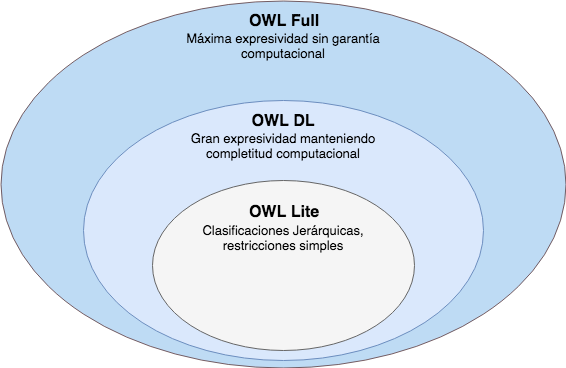
\includegraphics[width=150mm]{figuras/Diagramas-OwlSubClasses}
    \caption{Subclases OWL}
    \label{img:subclases owl}
    \end{figure}

OWL DL posee todas las características de OWL Lite más sus propias complejidades. OWL Full posee las mismas características de OWL DL agregando otras que resultan en mayor complejidad.
